\documentclass[10pt,a4paper]{article}
\usepackage[margin=2.2cm]{geometry}
\usepackage{longtable,booktabs,array,graphicx,xcolor,float,caption,enumitem}
\usepackage[hidelinks]{hyperref}
\usepackage[T1]{fontenc}
\usepackage{lmodern}
\usepackage{microtype}
\definecolor{osdag}{RGB}{105,145,20}
\definecolor{failc}{RGB}{190,30,30}
\definecolor{passc}{RGB}{30,120,50}
\newcommand{\gh}[1]{\href{https://github.com/Nidhikhare12/OsdagBridge/issues/#1}{\##1}}
\newcommand{\no}{\textcolor{failc}{\textbf{no}}}
% issue numbers of the reports posted last (filled in when posted)
\newcommand{\issPF}{\gh{145}}   % partial factors ignored
\newcommand{\issCS}{\gh{146}}   % check switches ignored
\newcommand{\issBL}{\gh{156}}   % bearing length / construction stage
\newcolumntype{L}[1]{>{\raggedright\arraybackslash}p{#1}}
\setlength{\parindent}{0pt}
\setlength{\parskip}{5pt}
\setlength{\tabcolsep}{4pt}
\renewcommand{\arraystretch}{1.15}
\captionsetup{font=small,labelfont=bf}
\setcounter{tocdepth}{2}

\title{\textbf{OsdagBridge Software Testing \& Issue Reporting}\\[4pt]
\large Short-span steel plate girder bridge module\\[2pt]
\normalsize FOSSEE Winter Internship 2026 screening task}
\author{Mounil Hiren Kankhara}
\date{18 November 2026}

\begin{document}
\maketitle

\begin{center}
\begin{tabular}{@{}ll@{}}
Repository under test & \url{https://github.com/Nidhikhare12/OsdagBridge} (branch \texttt{dev}, commit \texttt{d74f56d})\\
Test logs, scripts and notes & \url{https://github.com/Mounil2005/OsdagBridge} (branch \texttt{task-testing})\\
Issues raised & \gh{64}--\gh{70}, \gh{84}, \gh{140}--\gh{144}, \issPF, \issCS, \issBL\\
Comments on existing issues & \gh{68}, \gh{132}, \gh{142}\\
Screencast & link in the submission form (file \texttt{OsdagBridge\_Testing\_Workflow.mp4})
\end{tabular}
\end{center}

\section*{Summary}
33 test cases were executed: 30 at the code level (the design pipeline driven from a script, with the input and output dictionaries compared before and after every run) and 3 through the desktop application (custom materials and three consecutive runs, recorded on video). 16 GitHub issues were raised, each with the trigger conditions, evidence, the root cause in the source and a suggested change, and 3 comments were added to existing issues. No issue was posted where an existing one already covered the same problem.

The findings fall into four groups:
\begin{itemize}[nosep]
\item \textbf{Loads that do not reach the analysis.} The impact factor is always 0.10 (\gh{140}); the transverse wind area leaves out the girder and the force is applied twice (\gh{141}); the vehicles ticked in the Loading tab are ignored (\gh{142}); the crash barrier and median loads use fixed defaults (\gh{143}); the footpath pressure is ignored and treated as dead load (\gh{144}).
\item \textbf{Inputs that are saved but not used.} Partial safety factors $\gamma_c$, $\gamma_s$, $\gamma_{fl}$ and the self-weight factor (\issPF), the check on/off switches (\issCS), the bearing length and the construction-stage option (\issBL). In each case a control run with an input that \emph{is} used ($\gamma_{m0}$) showed that the method detects a change.
\item \textbf{Validation and data handling.} An empty span passes the file validator (\gh{67}); \texttt{design()} accepts spans outside 20--45~m (\gh{69}); \texttt{design()} rewrites 35 input keys from mm to m (\gh{66}); the railing load and crash barrier area differ between the defaults and the dialog (\gh{64}, \gh{84}).
\item \textbf{Report content.} ``Design pass'' next to a failing design (\gh{65}), blank or N/A load values (\gh{68}), missing units and symbols (\gh{70}).
\end{itemize}
Repeated designs on the same bridge object were stable in every case tried (Section~\ref{sec:multi}).

\tableofcontents
\newpage

\section{Introduction and Setup}
\textbf{Module under test:} the plate girder bridge design of OsdagBridge: input dialogs, grillage analysis, design checks, 3D CAD model, plots and the PDF report.

\textbf{Environment.} Windows 11, Python 3.12 in the \texttt{osdagbridge-env} conda environment created from \texttt{environment.yml}, MiKTeX 25.12 for the report. The fork was cloned with \texttt{upstream} set to the task repository and \texttt{dev} updated with \texttt{git pull upstream dev --rebase}; all results are on commit \texttt{d74f56d}. The application was started with \texttt{python -m osdagbridge.desktop}.

\textbf{Baseline design.} Highway bridge, span 30~m, carriageway 7.5~m, no median, no footpath, location Ahmedabad (Gujarat), design type Optimized; the layout solver gives four girders at 2.1~m, deck 250~mm, overhang 1.05~m; girder \texttt{E 350A}, deck \texttt{M40}, crash barrier \texttt{IRC 5 -- RCC Crash Barrier}. Saved as \texttt{osi\_files/TC-baseline\_inputs.osi}. Every case changes only the parameters listed for it.

\section{Test Methodology}
\textbf{Level 1, code level.} \texttt{testing\_scripts/run\_case.py} loads an \texttt{.osi} file, applies the values a user would type (\texttt{--set}, or \texttt{--after} for values the user edits after the layout has been derived), derives the dependent inputs with the same solver the GUI uses, and runs \texttt{design()}. For each run it stores the input dictionary before and after the design, the full output dictionary (about 1\,060 keys), the eight governing utilisations and the solver log; with \texttt{--fresh} it also repeats every run on a new object and compares the two (stale-state check). Files are in \texttt{evidence/}.

\textbf{Level 2, GUI level.} Custom steel and concrete were entered in the dialogs, the design was run, unlocked, edited and run again twice; the 3D model and plots were opened after each run. The session was recorded, and the input saved after each run was also passed through the Level 1 script.

\textbf{Checking that an input is used.} For each Additional Inputs field, the source was searched for code that reads its key. Every field that looked unused was then changed to a clearly different value and the design re-run: if all outputs stayed identical, the input is not used. A control run with an input that is known to be used ($\gamma_{m0}$ 1.10~$\rightarrow$~1.20) changed flexure from 19.51 to 21.08~\%, which shows that the comparison detects a real change.

\textbf{Checking calculation functions.} Code clause functions were called directly over a range of inputs (for example the impact factor for spans 10--45~m) and compared with the clause and with the other values the program prints. Where a function was suspect, the design was re-run once with the function temporarily corrected, the outputs compared, and the source restored (\texttt{git status} clean afterwards).

\textbf{Duplicates.} Before each issue, all open and closed issues of the repository (more than 140) were searched by keyword, and the candidate was dropped if an existing issue already covered it. Where an existing issue is related, the new one says what it adds.

\textbf{Pass/fail rule.} PASS when the design completes, the values entered are used, and the dictionaries and report agree with the inputs. FAIL for an error, an accepted invalid input, an input that has no effect, or a mismatch between UI, dictionary, analysis and report. Fatigue utilisation above 100~\% appears in most cases; it is a design result already tracked in \gh{44}.

\section{Test Cases}
The complete log (exact parameters, custom-property flags, run number, expected and actual results, dictionary checks, CAD and plot status, issue link, evidence file) is \texttt{test\_case\_log.csv}.

\subsection{Passing cases}
\begin{longtable}{@{}L{1.25cm}L{4.6cm}L{5.2cm}L{5.4cm}@{}}
\toprule
\textbf{ID} & \textbf{Parameters changed} & \textbf{Result} & \textbf{Notes}\\
\midrule\endfirsthead
\toprule \textbf{ID} & \textbf{Parameters changed} & \textbf{Result} & \textbf{Notes}\\ \midrule\endhead
TC-002 & span 20 (minimum) & completes; flexure 25.3\,\%, shear 38.2\,\% & fatigue 220.9\,\% (\gh{44})\\
TC-003 & span 45, carriageway 12 & completes; flexure 19.0\,\%, shear 57.4\,\% & fatigue 160.1\,\% (\gh{44})\\
TC-006 & skew 10$^{\circ}$ & completes; shear 42.2\,\% & values differ from baseline as expected\\
TC-007 & include median & completes; shear 80.9\,\% & median load: see TC-027\\
TC-008 & custom steel (fy 410, fu 540) and custom deck concrete (fck 35, fctm 2.8, Ecm 32) & completes; flexure 17.1\,\% against 19.5\,\% with default steel & custom steel is applied\\
TC-009 & three runs on one object: span 30, 25, 35 with carriageway 9 & each run equals a fresh run & Section~\ref{sec:multi}\\
TC-011 & deck overhang 0 & completes (shear 95.7\,\%) & upstream report Aditya-Donde \#440 does not reproduce here\\
TC-012 & GUI: custom steel and concrete & values kept, design completes & CAD and plots shown (video)\\
TC-013 & GUI run 2: span 24 & completes; values update & no stale data\\
TC-014 & GUI run 3: span 28, carriageway 8.5 & completes; values update & no stale data\\
TC-015 & two runs, carriageway 10.5 (stored 4-girder layout) & identical runs, equal to fresh & \\
TC-016 & span 20 with carriageway 20, then span 25 & run 2 equals a fresh run & \\
TC-017 & skew $+15^{\circ}$ & completes; shear 41.73\,\% & compare TC-018\\
TC-019 & two runs, carriageway 10.5, layout derived by the app (5 girders) & identical runs, equal to fresh & \gh{135} not reproduced with this layout\\
TC-029 & control: $\gamma_{m0}$ 1.20 & flexure 19.51 $\rightarrow$ 21.08\,\% & input is used\\
\bottomrule
\end{longtable}

\subsection{Failing cases}
\begin{longtable}{@{}L{1.25cm}L{3.8cm}L{7.3cm}L{4.1cm}@{}}
\toprule
\textbf{ID} & \textbf{Parameters} & \textbf{Observed} & \textbf{Issue}\\
\midrule\endfirsthead
\toprule \textbf{ID} & \textbf{Parameters} & \textbf{Observed} & \textbf{Issue}\\ \midrule\endhead
TC-001 & baseline, GUI report & report: girder dimensions in m labelled mm; ``design pass'' while status is Fail; blank/N/A loads; missing units; railing load 1.4715 in input, 6.806 in report; crash barrier 0.00~MT & \gh{64}, \gh{65}, \gh{66}, \gh{68}, \gh{70}, \gh{84}\\
TC-004/005 & span 19.9 / 45.1 & \texttt{design()} completes; the validator rejects the same values & \gh{69}\\
TC-010 & empty span in \texttt{.osi} & validator says valid, then \texttt{ValueError} & \gh{67}\\
TC-018 & skew $-15^{\circ}$ & shear 53.27\,\% against 41.73\,\% at $+15^{\circ}$ & existing \gh{132} (reproduced, comment added)\\
TC-020 & 7 girders forced on a 5-girder layout & run 1 \texttt{AttributeError}, run 2 completes; input internally inconsistent & inconclusive, not filed\\
TC-021/022 & only Class A / no vehicle ticked & identical to baseline; governing live load still Class 70R & \gh{142}\\
TC-023 & impact factor temporarily set to Cl.~208.2 value & live moment +9.7\,\%, deflection 9.64 $\rightarrow$ 10.58~mm, stud spacing and deck steel change; shipped value is 0.10 for all spans & \gh{140}\\
TC-024 & wind on baseline & FT = 14.79~kN, i.e.\ A1 = deck slab only; applied to both outer girders & \gh{141}\\
TC-025/026 & footpath both sides; custom pressure 1.0 & 4.905~kN/m$^2$ in both runs, added to the dead-load case & \gh{144}\\
TC-027 & crash barrier, median & analysis 6.54 and 4.00~kN/m against 7.557 and 14.08~kN/m in the inputs & \gh{143}\\
TC-028/030 & $\gamma_c$ 1.8, $\gamma_s$ 1.3, $\gamma_{fl}$ 1.5; self-weight factor 1.5 & identical to baseline & \issPF\\
TC-031 & fatigue, bending, deflection checks off & checks still run; status Fail on fatigue & \issCS\\
TC-032/033 & bearing length 100~mm; construction stage No & identical to baseline & \issBL\\
\bottomrule
\end{longtable}

\section{UI vs Input/Output Dictionary Comparison}
\subsection{Input dictionary against the values entered}
For the baseline, the 576 keys of the input dictionary were compared with the values saved from the UI, before and after \texttt{design()}. Scalar inputs are identical before the design; 35 girder dimension keys are rewritten in metres by \texttt{design()}.

\begin{table}[H]
\centering\small
\begin{tabular}{@{}L{5.6cm}L{2.2cm}L{2.3cm}L{2.2cm}L{3.6cm}@{}}
\toprule
\textbf{Input key (UI field)} & \textbf{UI value} & \textbf{Dict before design} & \textbf{Dict after design} & \textbf{Match}\\
\midrule
geometry.span / carriageway\_width & 30 / 7.5 & 30 / 7.5 & 30 / 7.5 & yes\\
typical\_section.no\_of\_girders / girder\_spacing & 4 / 2.1 & 4 / 2.1 & 4 / 2.1 & yes\\
material.girder fy / fu (MPa) & 350 / 490 & 350 / 490 & 350 / 490 & yes\\
material.deck / fck (MPa) & M40 / 40 & M40 / 40 & M40 / 40 & yes\\
crash\_barrier.area & (default) & 302282.768 mm$^2$ & same & dialog writes m$^2$ (\gh{84})\\
railing.load\_value (kN/m) & (default) & 1.4715 & 1.4715 & report shows 6.806 (\gh{64})\\
section\_input.depth (mm) & 1670 & 1670 & \textbf{1.67} & \no{} (\gh{66})\\
section\_input.bottom\_flange\_width (mm) & 510 & 510 & \textbf{0.51} & \no{} (\gh{66})\\
\bottomrule
\end{tabular}
\caption{Baseline: input dictionary against the UI values.}
\end{table}

\subsection{Values the analysis actually uses}
The solver log and the output dictionary show which value of an input reaches the analysis. Several inputs are stored correctly but a different value is used:

\begin{table}[H]
\centering\small
\begin{tabular}{@{}L{4.6cm}L{3.9cm}L{4.4cm}L{2.8cm}@{}}
\toprule
\textbf{Quantity} & \textbf{Input dictionary / report} & \textbf{Used in the analysis} & \textbf{Issue}\\
\midrule
Impact factor, Class A, 30~m & 1.207 (report Ch.~3) & 1.10 for every vehicle & \gh{140}\\
Transverse wind area A1 & girder + deck + barrier & deck slab only, 7.5~m$^2$; force on both outer girders & \gh{141}\\
Vehicles & ticked in Loading tab & always Class A / 70R from width & \gh{142}\\
Crash barrier load & 7.557~kN/m & 6.54~kN/m & \gh{143}\\
Median load & 14.08~kN/m & 4.00~kN/m & \gh{143}\\
Footpath pressure (Custom) & 1.0~kN/m$^2$ & 4.905~kN/m$^2$ as dead load & \gh{144}\\
$\gamma_c$, $\gamma_s$, $\gamma_{fl}$, self-weight factor & as entered (report Ch.~2) & fixed 1.50, 1.15, --, 1.00 & \issPF\\
Check switches & off & all checks run & \issCS\\
Bearing length, construction stage & 100~mm, No & automatic, checked & \issBL\\
\bottomrule
\end{tabular}
\caption{Inputs stored correctly but not used as entered.}
\end{table}

For the custom-material cases (TC-008, TC-012 to TC-014) the custom steel and concrete values are kept and used: flexure falls from 19.5 to 17.1~\% with the stronger steel. The known problems with custom densities and grades (\gh{19}, \gh{20}, \gh{41}, \gh{43}) were not repeated.

\subsection{Output dictionary against the report and the docks}
\begin{table}[H]
\centering\small
\begin{tabular}{@{}L{4.4cm}L{4.4cm}L{5.0cm}L{2.0cm}@{}}
\toprule
\textbf{Item} & \textbf{Output dictionary} & \textbf{Report / Results Table} & \textbf{Match}\\
\midrule
Span, carriageway & 30, 7.5 & 30 m, 7.5 m & yes\\
Overall status & fatigue 157.26\,\% & ``Fail (Fatigue Normal Stress)'' & yes\\
Executive Summary outcomes & fatigue fails & every component ``design pass'' & \no{} (\gh{65})\\
Girder depth & 1670~mm & ``1.67 mm'' & \no{} (\gh{66})\\
Lanes, braking, seismic force & not in saved input; braking function raises & blank or N/A & \no{} (\gh{68})\\
Crash barrier weight & 45.34~MT expected & 0.00~MT & \no{} (\gh{84})\\
Flexure, Results Table & 2219.12 / 11371.85~kNm & same values, UR 0.20 & yes\\
Reinforcement stress, Results Table & 365.35 / 358.89~MPa & same values & yes\\
\bottomrule
\end{tabular}
\caption{Baseline: output dictionary against the report and the Results Table.}
\end{table}

All 37 Results Table builders were run on the baseline design without errors and the table-to-builder mapping was checked. The remaining differences there (live deflection, wind speed, Excel units, overall width) are already reported in \gh{114}, \gh{86}, \gh{82} and \gh{124}.

\begin{figure}[H]
\centering
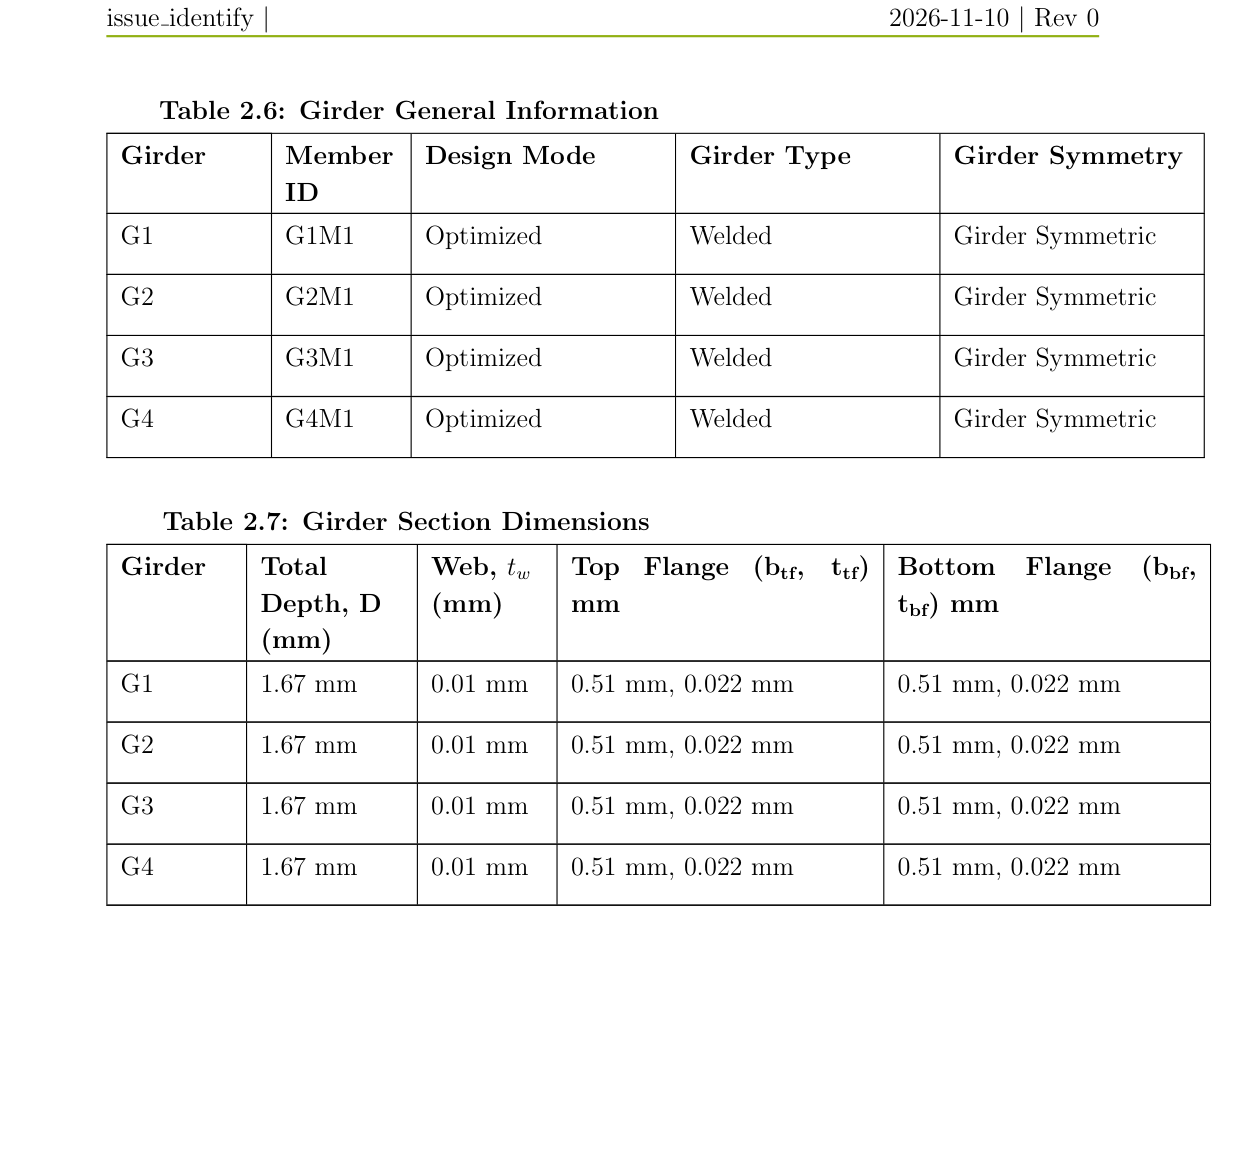
\includegraphics[width=0.8\textwidth]{issue_images/report_p10_section_dims.png}
\caption{Report ``Girder Section Dimensions'' table with metres under an mm heading (\gh{66}).}
\end{figure}

\section{Multi-Run Stability}\label{sec:multi}
\begin{table}[H]
\centering\small
\begin{tabular}{@{}L{1.5cm}L{6.2cm}rrrr@{}}
\toprule
\textbf{Case} & \textbf{Runs on one object} & \textbf{Flexure \%} & \textbf{Shear \%} & \textbf{LTB \%} & \textbf{Fatigue \%}\\
\midrule
TC-009 & 1: span 30 & 19.51 & 39.91 & 22.81 & 157.26\\
 & 2: span 25 & 23.80 & 57.73 & 19.71 & 199.16\\
 & 3: span 35, carriageway 9 & 19.05 & 56.49 & 28.23 & 150.50\\
TC-016 & 1: span 20, carriageway 20 & 64.99 & 102.73 & 56.00 & 573.86\\
 & 2: span 25 & 55.86 & 146.31 & 42.76 & 484.44\\
TC-019 & 1 and 2: carriageway 10.5 (5 girders) & 23.06 & 48.75 & 24.44 & 187.06\\
TC-012--014 & GUI runs 1--3 (span 30, 24, 28 / cw 8.5) & 17.14 / 20.95 / 20.91 & 39.91 / 53.79 / 75.34 & 22.50 / 17.41 / 22.35 & 157.26 / 196.76 / 192.66\\
\bottomrule
\end{tabular}
\caption{Consecutive runs. In every scripted case each run equals the same run on a fresh object; no error.}
\end{table}

\textbf{Observations.} No stale values were carried from one run to the next in any scripted case, and in the GUI the inputs, cross-section drawing, output dock, 3D model and plots were updated after each unlock and re-design, without a crash or frozen window. Two upstream reports on repeated runs were checked: \gh{135} (crash on a second \texttt{design()}) was not reproduced with the layout the app derives for a 10.5~m carriageway (5 girders); forcing 7 girders onto that layout raised an \texttt{AttributeError} on the first run only, but that input is internally inconsistent, so it was not filed. \gh{85} (empty 3D view after unlock) concerns the GUI viewer and was not reproduced in the recorded session, which used narrower carriageways.

\section{3D CAD and Plot Verification}
\begin{itemize}[nosep]
\item \textbf{3D CAD:} deck, girders, bracing and both crash barriers are drawn; the deck length and width follow the inputs in each run (span 24 in run 2; span 28 with carriageway 8.5 in run 3). Layer check boxes (Bridge, Girder, Deck, Cross Bracing, Crash Barrier) are shown above the model.
\item \textbf{Plots:} the deflection and bending moment diagrams for a selected member and load case open from the output dock after the last run, one curve per girder.
\end{itemize}
Visual accuracy was judged by comparing the geometry with the inputs; plotted values were not recomputed independently.

\begin{figure}[H]
\centering
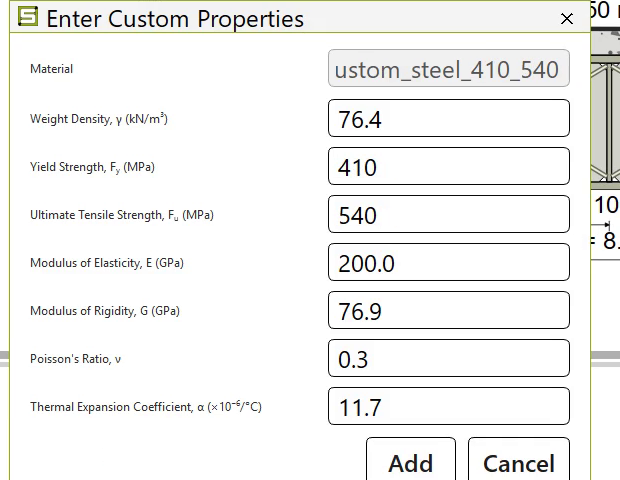
\includegraphics[width=0.46\textwidth]{video_frames/custom_steel_dialog.png}\hfill
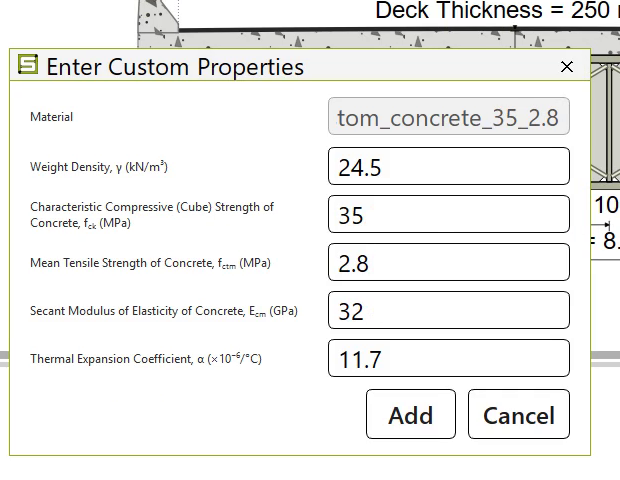
\includegraphics[width=0.46\textwidth]{video_frames/custom_concrete_dialog.png}
\caption{Custom properties entered for the girder steel (fy 410, fu 540) and the deck concrete (fck 35, fctm 2.8, Ecm 32).}
\end{figure}
\begin{figure}[H]
\centering
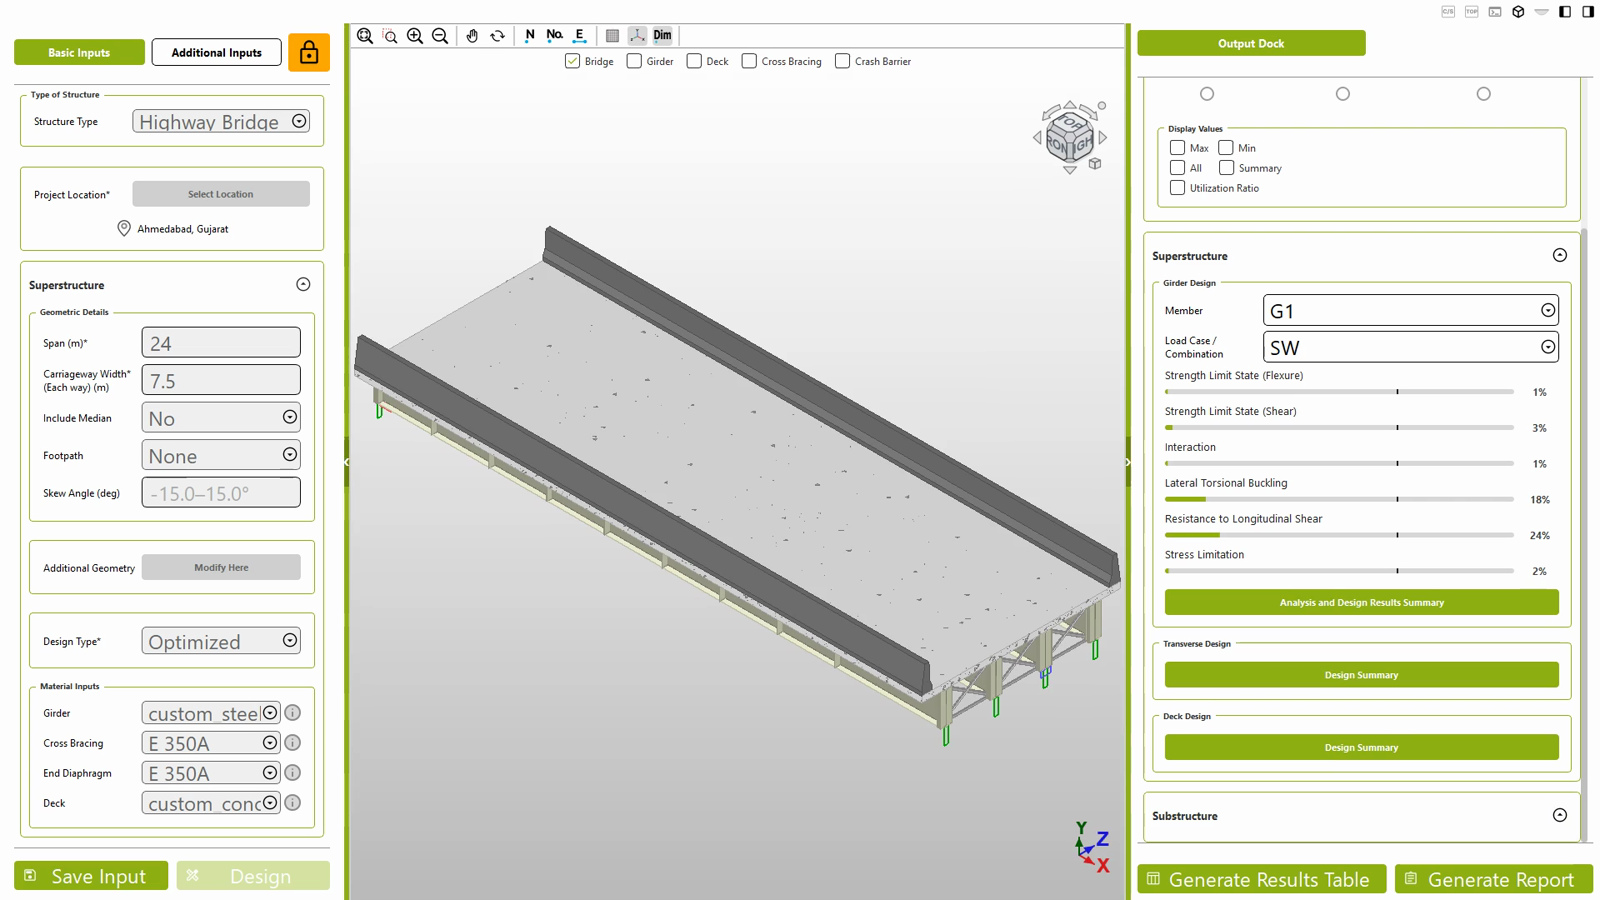
\includegraphics[width=0.48\textwidth]{video_frames/frame_100s.png}\hfill
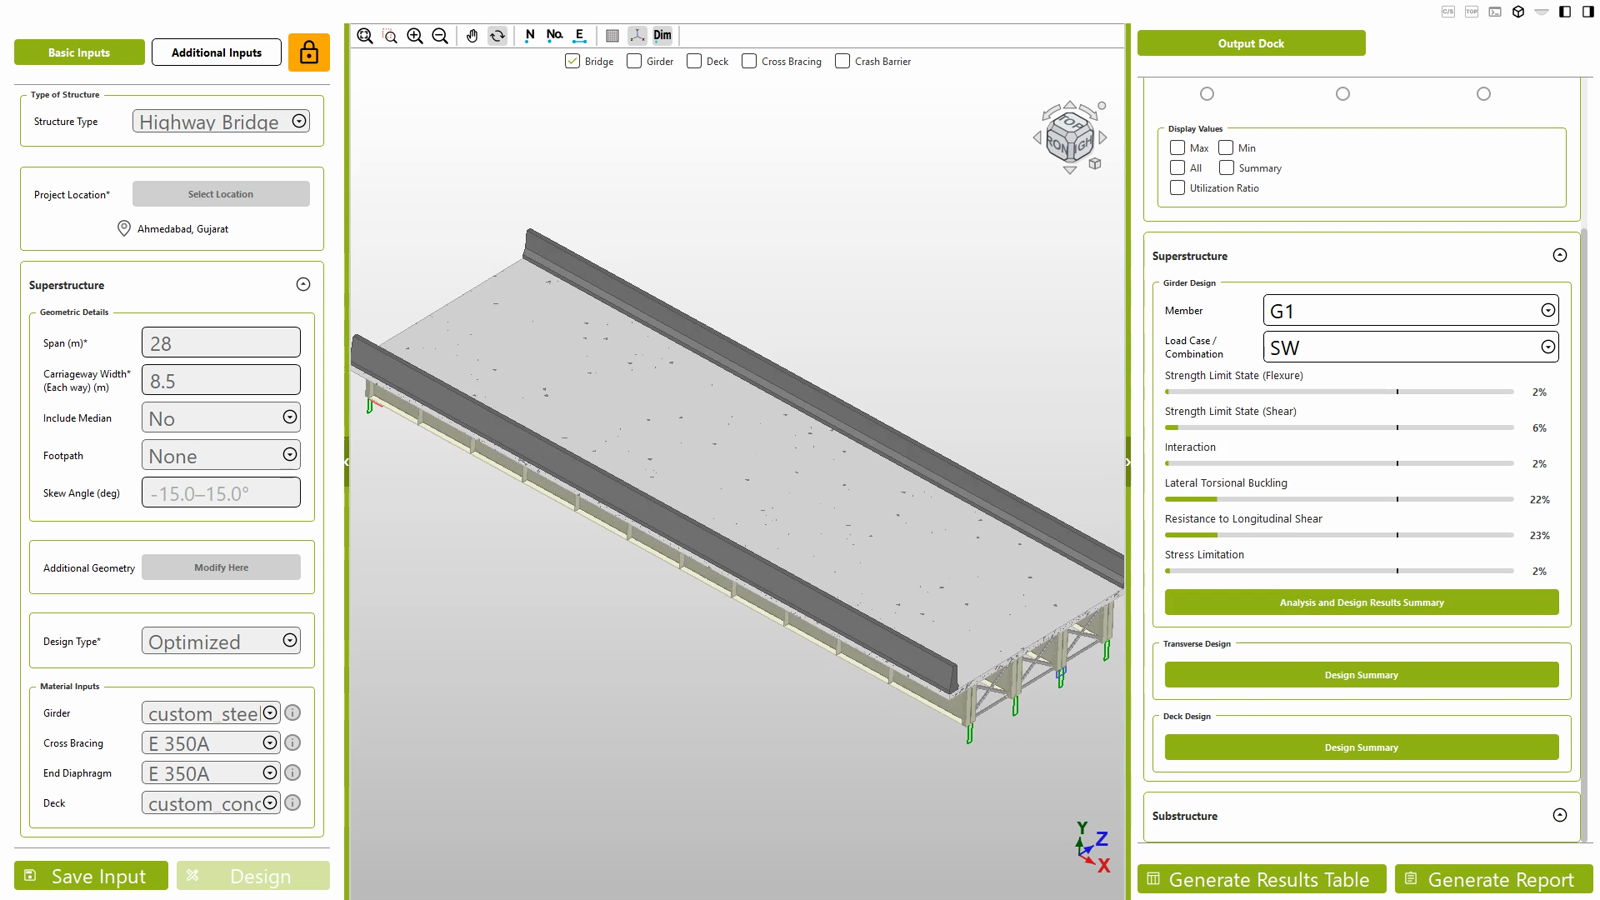
\includegraphics[width=0.48\textwidth]{video_frames/frame_150s.png}
\caption{3D model after run 2 (span 24) and run 3 (span 28, carriageway 8.5).}
\end{figure}
\begin{figure}[H]
\centering
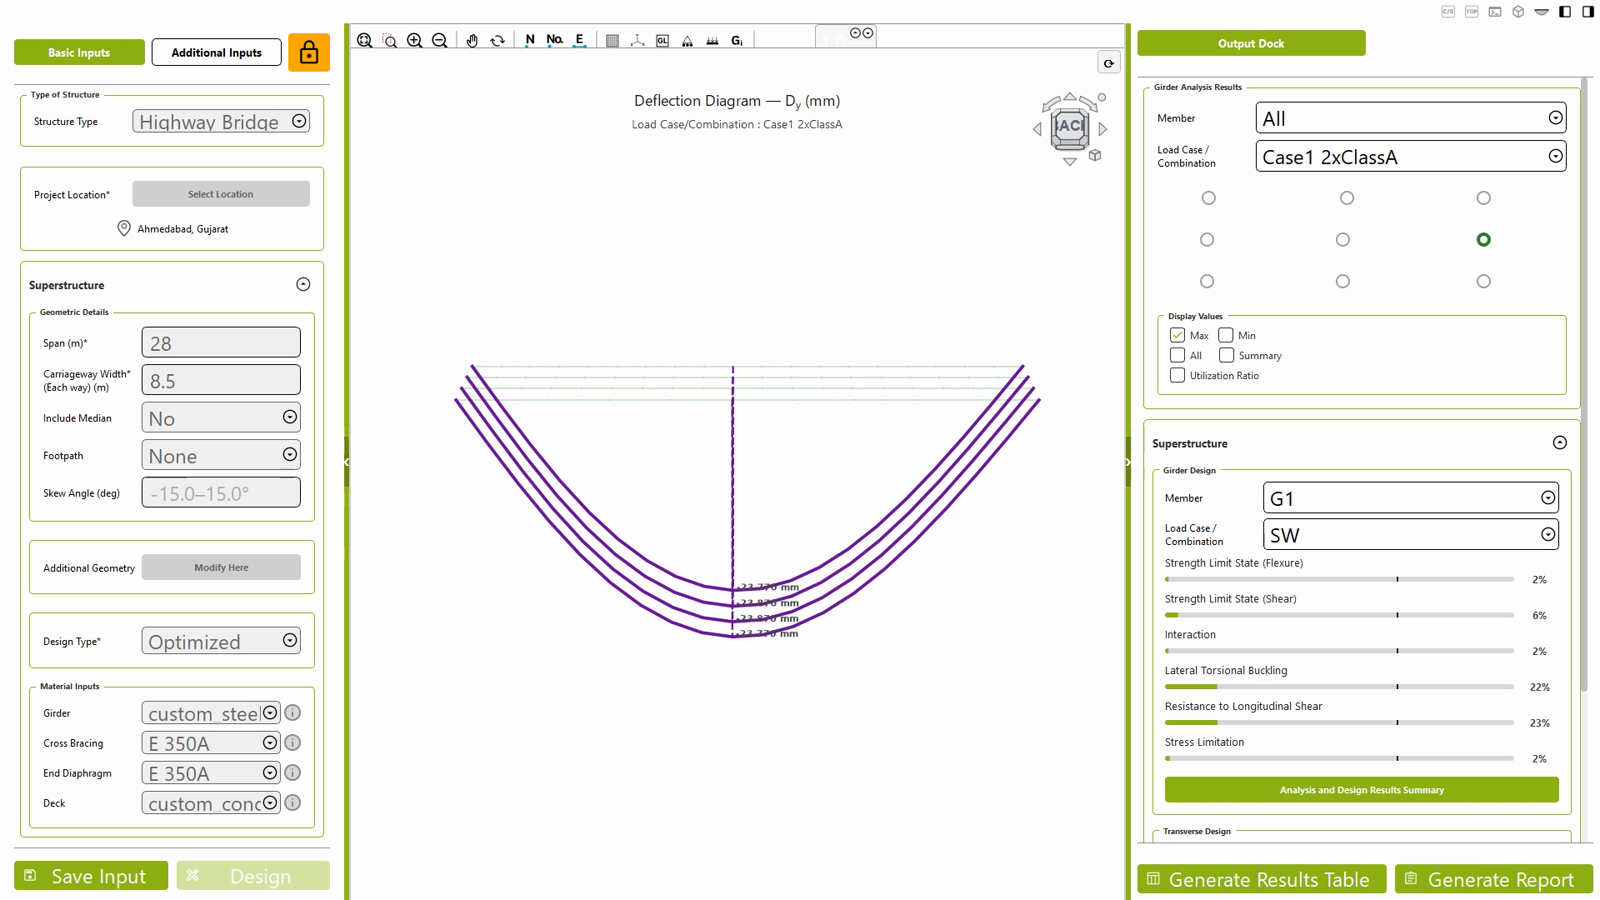
\includegraphics[width=0.58\textwidth]{video_frames/frame_178s.png}
\caption{Deflection diagram of the final run.}
\end{figure}

\section{Issues Raised}
\begin{longtable}{@{}L{1.1cm}L{7.0cm}L{7.5cm}@{}}
\toprule
\textbf{Issue} & \textbf{Problem} & \textbf{Root cause and files}\\
\midrule\endfirsthead
\toprule \textbf{Issue} & \textbf{Problem} & \textbf{Root cause and files}\\ \midrule\endhead
\gh{140} & impact factor always 0.10; applied to Class A, report shows 1.207 & \texttt{irc6\_2017.py} \texttt{cl\_208\_3\_impact\_factor} tests the constant \texttt{KEY\_VEHICLE[1]}; \texttt{analyser.py} line 1803\\
\gh{141} & transverse wind area excludes the girder; force applied to both outer girders & \texttt{irc6\_2017.py} lines 681--685; \texttt{analyser.py} lines 1437, 1456--1466\\
\gh{142} & Loading-tab vehicle selection ignored & \texttt{analyser.vehicle\_lane\_coordinates()}, \texttt{deckdesign.\_governing\_vehicle()}\\
\gh{143} & crash barrier and median loads use fixed defaults & key \texttt{"crash\_barrier\_load"} in \texttt{crash\_barrier/geometry.py}; \texttt{create\_median\_load()} called without value\\
\gh{144} & custom footpath pressure ignored; pedestrian load in dead load & \texttt{analyser.create\_footpath\_load()}, \texttt{create\_dead\_load\_combination()}\\
\issPF & $\gamma_c$, $\gamma_s$, $\gamma_{fl}$, self-weight factor not used & fixed values in \texttt{irc22\_2015.py} lines 41, 401, 412\\
\issCS & check on/off switches not used & \texttt{design\_options\_cont.uls.*}/\texttt{sls.*} never read\\
\issBL & bearing length and construction stage not used & \texttt{designer.py} \texttt{bs\_b1\_mm} never set\\
\gh{64} & railing load 1.4715 in input, 6.806 in design and report & two formulas for one key: \texttt{defaults.py}, \texttt{additional\_inputs.py}\\
\gh{65} & ``design pass'' while the design fails & hard-coded text in \texttt{executive\_summary.py}\\
\gh{66} & girder dimensions in m under an mm heading & in-place conversion in \texttt{plategirderbridge.py}; \texttt{chap2.py}\\
\gh{67} & empty span passes validation, then \texttt{ValueError} & validator accepts empty string; \texttt{defaults.py} line 531\\
\gh{68} & blank or N/A load values in the report & keys not saved; computed strings unused; braking function raises (comment)\\
\gh{69} & \texttt{design()} accepts spans outside 20--45~m & range check only in UI and file validator\\
\gh{70} & missing units and dropped $\le$ in the Executive Summary & \texttt{executive\_summary.py}; \texttt{\_tex()}\\
\gh{84} & crash barrier 0.00~MT in the take-off & mm$^2$ in defaults, m$^2$ in the dialog; \texttt{boq\_generator.py}\\
\bottomrule
\end{longtable}

\textbf{Comments added:} \gh{68} (\texttt{cl\_211\_2\_braking\_force} raises \texttt{UnboundLocalError} for every lane count), \gh{132} (skew asymmetry reproduced on Windows: shear 41.73 against 53.27~\%), \gh{142} (the dialog text says only ticked vehicles are analysed).

\section{Conclusion}
The design pipeline is stable: no crash in any valid case, results respond correctly to geometry and material changes, custom materials are applied, and repeated designs on the same object give the same results as fresh ones. The main weakness is the path from inputs to the analysis: several loads and options are stored and printed in the report but not used, so the report can describe a different design from the one that was checked. Fixing \gh{140}--\gh{144} affects the live, wind and dead loads directly, and the unused inputs (\issPF, \issCS, \issBL) should either be connected or made read-only.

\textbf{Limits of this testing.} Only the plate girder bridge was tested; location was set by name; the custom load combination table, custom vehicles, the live-load eccentricity and the CAD export were not exercised. Engineering values were not re-derived by hand; the claims are about consistency between inputs, analysis, dictionaries and report, and about the code paths identified.

\textbf{Repository contents (branch \texttt{task-testing}):} \texttt{testing\_scripts/run\_case.py}, \texttt{run\_batch.sh}; \texttt{testing/test\_case\_log.csv}, \texttt{osi\_files/}, \texttt{evidence/}, \texttt{issue\_final/}, this report.

\end{document}
